\section{Introduction}
Task automation on smartphones aims to enable a mobile agent to autonomously execute tasks based on user-provided descriptions, thereby freeing the user's hands and enhancing the user experience. Recent studies have introduced various mobile agents driven by large language models (LLMs) \citep{wang2023enabling, wen2024autodroid, wang2024mobile, wang2025mobile, DBLP:conf/chi/ZhangYLLHCHF025, lee2024mobilegpt}. These agents operate in a human-like manner. Typically, they receive user commands, sequentially assess the page state, generate the corresponding sub-task, and determine how to interact with the graphical user interface (GUI) until the task is completed. 

In practice, most agents rely on cloud-based proprietary LLMs \citep{wang2023enabling, wen2024autodroid, lee2024mobilegpt}, such as GPT-4o accessed via OpenAI’s paid API. These models contain at least hundreds of billions of parameters and demonstrate powerful reasoning capabilities, enabling mobile agents to achieve high success rates on a variety of simple tasks. Despite the promising results, several limitations remain. In mobile automation tasks, the agent must capture the page information at every step and upload it to the cloud-based LLM. We find that the information uploaded for decision-making is excessive, with only a small portion being relevant and the rest redundant. For many sub-tasks executed on smartphone interfaces, the only required action is to click a functional button, which relies solely on the local information of specific UI elements rather than on the full page context. However, current mobile agents do not take advantage of this property, they routinely upload the complete page to the cloud-based LLM, thereby transmitting a large amount of redundant information that may even contain sensitive user data. As shown in Figure~\ref{fig:intro}, if the user query is to search something, only the search bar needs to be activated and other information on the page is superfluous. Smartphones have a privacy-sensitive nature and users are reluctant to expose their private information too much. 

One seemingly straightforward solution is to deploy open‑source LLMs locally, thereby avoiding any data exposure to the cloud. However, these models typically contain only billion-scale parameters and thus exhibit only elementary reasoning capabilities. Their performance on mobile automation tasks is poor, yielding low success rates and a substantial performance gap compared to cloud LLMs. 

To solve these problems, we propose \textbf{CORE}, a collaborative architecture that leverages both cloud-based strong LLMs and locally deployable light-weight LLMs. First, we employ a hierarchy‐guided strategy based on the XML tree structure to partition the page into structured blocks. Instead of uniform segmentation that disrupts inherent UI structures, the partitioning follows the original UI design intent and preserves logical element clusters. The next step is to locally rank the blocks by their importance to the current sub-task. The local LLM’s limited planning capability leads to inaccurate sub-task generation, which compromises the validity of the ranking. To remedy this, we design a collaborative planning module that combines the cloud LLM’s powerful planning ability with the local model’s basic reasoning capability and its advantage of full-page access. Specifically, the local LLM generates multiple candidate sub-tasks from different blocks. The cloud model, by comprehensively analyzing these candidates, indirectly infers the page context and selects the most plausible sub-task or generates a more accurate one. We further design a collaborative decision module that integrates the coarse-grained filtering of the local LLM with the fine-grained decision-making of the cloud LLM. The confirmed sub-task is fed back to the local LLM to guide block ranking. We pass the top-ranked block to the cloud LLM for element-wise decision-making. We also introduce a multi-round accumulation mechanism. If the cloud LLM considers the selected block insufficient for a proper decision, it will incrementally ask the local LLM for additional blocks until the provided information is judged to be adequate for a confident decision. This collaborative process achieves a dynamic balance between information sufficiency and reduction. These designs form a novel asymmetric collaborative framework, different from prior multi-agent approaches that typically employed cloud LLMs with distinct roles under full UI access. CORE establishes collaboration between a strong cloud LLM without direct UI access and a weak local LLM with full UI visibility but limited reasoning capability, coordinating by leveraging their complementary strengths.

\begin{figure}[!t]
    \centering
    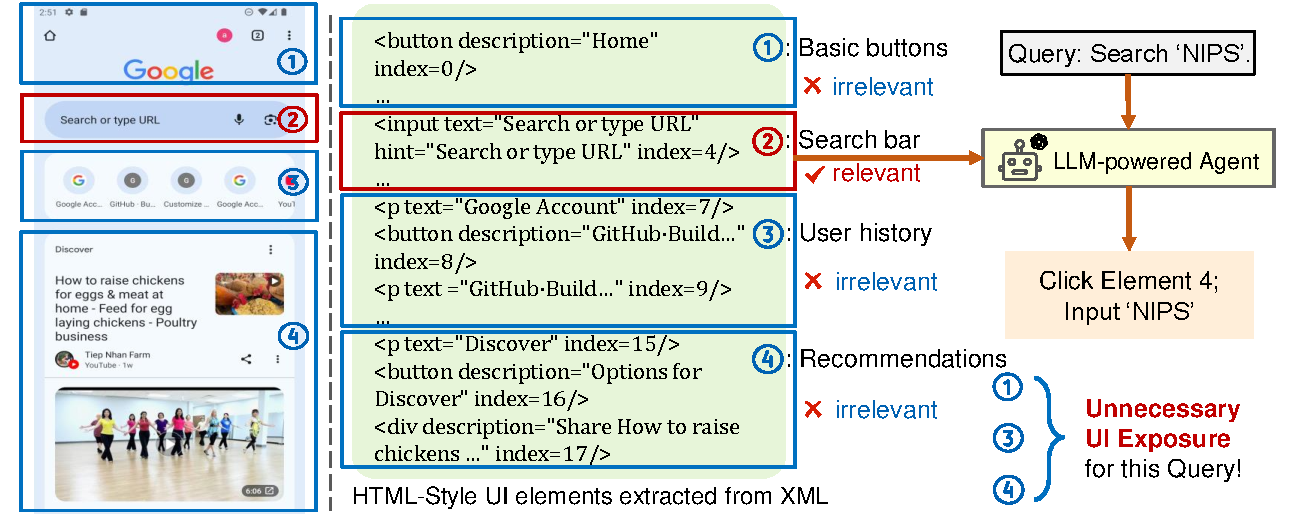
\includegraphics[width=0.95\textwidth]{pics/intro_v3.pdf}
    \caption{Given the user query ``Search NIPS'', only the search bar on the Chrome start page is task-relevant. Uploading just this block to the agent is sufficient for correct decision-making, indicating that other UI blocks (basic buttons, browsing history, recommendations) are unnecessary exposure.}\label{fig:intro}
    \vspace{-1.45em}
\end{figure}

Our main contributions are as follows: (1) To the best of our knowledge, we are the first to study the problem of reducing unnecessary information exposure and uploading only minimal sufficient UI contents to cloud-based LLMs during mobile agent's decision steps; (2) we propose an XML-based layout-aware block partitioning method to preprocess UI content, and a collaborative framework combining local and cloud LLMs for joint planning and decision-making, reducing UI exposure to the cloud while preserving decision accuracy; and (3) on the public DroidTask dataset (143 tasks, 12 apps) \citep{wen2024autodroid}, our GPT-4o + Gemma2-9B setup reduces UI exposure by 55.6\% with task success rate just 4.9\% lower than GPT-4o. On the public AndroidLab dataset (98 tasks, 9 apps) \citep{xu2024androidlab}, GPT-4o + Qwen2.5-7B achieves a 29.97\% reduction with only a 3.06\% drop, showing practical effectiveness. 
Moreover, CORE significantly reduces sensitive information exposure, lowering the number of sensitive UI elements uploaded to the cloud by 70.49\% on DroidTask and 38.84\% on AndroidLab.